\documentclass[12pt]{article}
 
\usepackage[margin=1in]{geometry} 
\usepackage{amsmath,amsthm,amssymb}
\usepackage{graphicx}
\usepackage{mathtools}
\usepackage{changepage}
\usepackage{listings}
\usepackage{caption}
\usepackage{float}
% \usepackage{minted}
% \setminted{baselinestretch=0.8}
\linespread{1.15}
\newenvironment{exercise}[2][Exercise]{\begin{trivlist}
\item[\hskip \labelsep {\bfseries #1}\hskip \labelsep {\bfseries #2.}]}{\end{trivlist}}
\renewcommand*{\proofname}{Solution}
\newenvironment{aw}
  {\begin{adjustwidth}{2em}{0em}}
  {\end{adjustwidth}}
\newcommand{\ro}{\text { or }}
\newcommand{\nd}{\text{ and }}



\begin{document}

% --------------------------------------------------------------
%
%                         Start here
%
% --------------------------------------------------------------

\title{Chapter 4: Relations} % replace with the problem you are writing up
\author{Saif Mohammed} % replace with your name
\maketitle

\section{Section 4.1: Ordered Pairs and Cartesian Products}

\begin{exercise}{5}
	Prove parts 2 and 3 of Theorem 4.1.3.
	\begin{aw}
		\textbf{Theorem 4.1.3.} Suppose $A$, $B$, $C$, and $D$ are sets.

		1. $A \times (B \cap C) = (A \times B) \cap (A \times C)$.

		2. $A \times (B \cup C) = (A \times B) \cup (A \times C)$.

		3. $(A \times B) \cap (C \times D) = (A \cap C) \times (B \cap D)$.

		4. $(A \times B) \cup (C \times D) \subseteq (A \cup C) \times (B \cup D)$.

		5. $A \times \emptyset = \emptyset \times A = \emptyset$.
	\end{aw}
\end{exercise}

\begin{proof}
	(2) Let $(x,y)\in A\times (B \cup C)$. So
	\begin{align*}
		           & x\in A \nd y\in B\cup C                                    \\
		\implies   & x\in A \nd (y\in B \ro y\in C)                             \\
		\implies   & (x\in A \nd y\in B) \ro (x\in A \nd y\in C )               \\
		\implies   & (x,y)\in A\times B \ro (x,y)\in A\times C                  \\
		\implies   & (x,y)\in (A\times B)\cup (A\times C)                       \\
		\therefore & \ A\times (B\cup C) \subseteq (A\times B)\cup (A\times C).
	\end{align*}

	Again, let $(x,y)\in (A\times B)\cup (A\times C)$. So
	\begin{align*}
		           & (x,y)\in A\times B \ro (x,y)\in A\times C                   \\
		\implies   & (x\in A \nd y\in B) \ro (x\in A \nd y\in C)                 \\
		\implies   & x\in A \nd (y\in B \ro y\in C)                              \\
		\implies   & x\in A \nd y\in B\cup C                                     \\
		\implies   & (x,y)\in A\times (B\cup C)                                  \\
		\therefore & \ (A\times B)\cup (A\times C)  \subseteq A\times (B\cup C).
	\end{align*}
	Hence, $A\times (B\cup C) = (A\times B)\cup (A\times C)$.

	(3) Let $(x, y) \in (A \times B) \cap (C \times D)$. So
	\begin{align*}
		           & (x, y) \in A \times B \nd (x, y) \in C \times D                          \\
		\implies   & (x \in A \nd y \in B) \nd (x \in C \nd y \in D)                          \\
		\implies   & (x\in A \nd x\in C) \nd (y\in B \nd y\in D)                              \\
		\implies   & x \in A \cap C \nd y \in B \cap D                                        \\
		\implies   & (x, y) \in (A \cap C) \times (B \cap D)                                  \\
		\therefore & \ (A \times B) \cap (C \times D) \subseteq (A \cap C) \times (B \cap D).
	\end{align*}

	Again, let $(x, y) \in (A \cap C) \times (B \cap D)$. So
	\begin{align*}
		           & x \in A \cap C \nd y \in B \cap D                                        \\
		\implies   & (x \in A \nd x \in C) \nd (y \in B \nd y \in D)                          \\
		\implies   & (x\in A \nd y\in B) \nd (x\in C \nd y\in D)                              \\
		\implies   & (x, y) \in A \times B \nd (x, y) \in C \times D                          \\
		\implies   & (x, y) \in (A \times B) \cap (C \times D)                                \\
		\therefore & \ (A \cap C) \times (B \cap D) \subseteq (A \times B) \cap (C \times D).
	\end{align*}
	Hence, $(A \times B) \cap (C \times D) = (A \cap C) \times (B \cap D)$.
\end{proof}

\begin{exercise}
	{6}
	What’s wrong with the following proof that for any sets \(A\), \(B\), \(C\), and \(D\), \((A \cup C) \times (B \cup D) \subseteq (A \times B) \cup (C \times D)\)? (Note that this is the reverse of the inclusion in part 4 of Theorem 4.1.3.)

	Proof. Suppose \((x, y) \in (A \cup C) \times (B \cup D)\). Then \(x \in A \cup C\) and \(y \in B \cup D\), so either \(x \in A\) or \(x \in C\), and either \(y \in B\) or \(y \in D\). We consider these cases separately.

	Case 1. \(x \in A\) and \(y \in B\). Then \((x, y) \in A \times B\).

	Case 2. \(x \in C\) and \(y \in D\). Then \((x, y) \in C \times D\).

	Thus, either \((x, y) \in A \times B\) or \((x, y) \in C \times D\), so \((x, y) \in (A \times B) \cup (C \times D)\). \(\qed\)
\end{exercise}

\begin{proof}
	There would be 4 cases. The other two cases are neglected in this proof. They are
	\begin{align*}
		    & x \in A \nd y \in D  \\
		\nd & x \in C \nd y \in B.
	\end{align*}
	That's why the proof is not correct. In fact, the statement is not correct at all. The correct statement will be
	\[
		(A\cup C)\times (B\cup D)\subseteq (A\times B)\cup (A\times D)\cup (C\times B)\cup (C\times B).
	\]
\end{proof}

\begin{exercise}
	{7}
	If \( A \) has \( m \) elements and \( B \) has \( n \) elements, how many elements does \( A\times B \) have?
\end{exercise}

\begin{proof}
	\( m\times n \).
\end{proof}

\begin{exercise}
	{8}
	Is it true that for any sets \( A \), \( B \), and \( C \), \( A \times (B \setminus C) = (A \times B) \setminus (A \times C) \)?
	Give either a proof or a counterexample to justify your answer.
\end{exercise}

\begin{proof}
	\begin{align*}
		           & (x,y) \in A\times (B \setminus C)                                 \\
		\implies   & x \in A \nd y \in B \nd y \notin C                                \\
		\implies   & (x \in A \nd y \in B) \nd (x \in A \nd y \notin C)                \\
		\implies   & (x,y) \in A\times B \nd (x,y) \notin A\times C                    \\
		\implies   & (x,y) \in (A\times B)\setminus (A\times C)                        \\
		\therefore & \ A \in (B\setminus C)\subseteq (A\times B)\setminus (A\times C).
	\end{align*}

	Again,
	\begin{align*}
		         & (x,y) \in (A\times B)\setminus (A\times C)      \\
		\implies & (x,y) \in A\times B \nd (x,y) \notin A\times C.
	\end{align*}

	Now there are three cases regarding \( (x,y)\notin A\times C \).

	\textbf{Case 1:} \( x\notin A \nd y \in C \). This case is contradictory to \( (x,y) \in A\times B \implies x \in A \nd y \in B \). So it is an invalid case.

	\textbf{Case 2:} \( x \notin A \nd y \notin C \). This is also invalid for the same reason as the 1st case.

	\textbf{Case 3:} \( x \in A \nd y \notin C \). This is the only valid case. Thus we can continue from the above equation:
	\begin{align*}
		           & (x,y) \in A\times B \nd (x,y) \notin A\times C                      \\
		\implies   & x \in A \nd y \in B \nd x \in A \nd y \notin C                      \\
		\implies   & x \in A \nd (y \in B \nd y \notin C)                                \\
		\implies   & x \in A \nd y \in (B\setminus C)                                    \\
		\implies   & (x,y)\in A\times (B\setminus C)                                     \\
		\therefore & \ (A\times B)\setminus (A\times C)\subseteq A\times (B\setminus C).
	\end{align*}
	Hence, \( A\times (B\setminus C)=(A\times B)\setminus (A\times C) \).
\end{proof}

\begin{exercise}
	{10}
	Prove that for any sets \( A \), \( B \), \( C \), and \( D \), \( (A \setminus C) \times (B \setminus D) \subseteq (A \times B) \setminus (C \times D) \).
\end{exercise}

\begin{proof}
	\begin{align*}
		           & (x,y)\in (A\setminus C)\times (B\setminus D)                                     \\
		\implies   & x\in A\setminus C \nd y\in B\setminus D                                          \\
		\implies   & x\in A \nd x\notin C \nd y\in B \nd y\notin D                                    \\
		\implies   & x\in A\nd y\in B\nd x\notin C\nd y\notin D                                       \\
		\implies   & (x,y)\in A\times B\nd (x,y)\notin C\times D                                      \\
		\implies   & (x,y)\in (A\times B)\setminus (C\times D)                                        \\
		\therefore & \ (A\setminus C)\times (B\setminus D)\subseteq (A\times B)\setminus (C\times D).
	\end{align*}
\end{proof}

\begin{exercise}
	{11}
	Prove that for any sets \( A \), \( B \), \( C \), and \( D \), \( (A \times B) \setminus (C \times D) = [A \times (B \setminus D)] \cup [(A \setminus C)\times B] \) .
\end{exercise}

\begin{proof}
	\begin{align*}
		\text{ Let } & (x,y)\in (A \times B) \setminus (C \times D)                                                          \\
		\implies     & (x,y)\in A\times B \nd (x,y)\notin C\times D                                                          \\
		\implies     & (x\in A \nd y\in B) \nd (x\notin C \ro y\notin D)                                                     \\
		\implies     & (x\in A \nd x\notin C \nd y\in B) \ro (x\in A \nd y\in B \nd y\notin D)                               \\
		\implies     & (x,y)\in [(A\setminus C)\times B]\cup [A\times (B\setminus D)]                                        \\
		\therefore   & \quad (A\times B)\setminus (C\times D)\subseteq [A\times (B\setminus D)]\cup [(A\setminus C)\times B]
	\end{align*}

	Again, for \( (x,y)\in [A\times (B\setminus D)]\cup [(A\setminus C)\times B] \), there are two cases.

	\textbf{Case 1:} \( (x,y)\in A\times (B\setminus D) \). It implies that \( y\notin D \). So we can say \( (x,y)\notin C\times D \).

	\textbf{Case 2:} \( (x,y)\in (A\setminus C)\times B \). It implies that \( x\notin C \). So we can say \( (x,y)\notin C\times D \).

	Hence, \( (x,y)\in (A\times B)\setminus (C\times D) \) and so \( [A\times (B\setminus D)]\cup [(A\setminus C)\times B]\subseteq (A\times B)\setminus (C\times D) \)

	Therefore, \( (A\times B)\setminus (C\times D)=[A\times (B\setminus D)]\cup [(A\setminus C)\times B] \).
\end{proof}

\begin{exercise}
	{12}
	Prove that for any sets \( A \), \( B \), \( C \), and \( D \), if \( A \times B \) and \( C \times D \) are disjoint, then either \( A \) and \( C \) are disjoint or \( B \) and \( D \) are disjoint.
\end{exercise}

\begin{proof}
	We need to prove that if \( (A\times B)\cap (C\times D)=\emptyset \), then either \( A\cap C=\emptyset \) or \( B\cap D=\emptyset \).
	\begin{align*}
		         & (A\times B)\cap (C\times D)=\emptyset &                                  \\
		\implies & (A\cap C)\times (B\cap D)=\emptyset   & \text{ [by Theorem 4.1.3 (3).] }
	\end{align*}
	Then by Theorem 4.1.3 (5), either \( A\cap C=\emptyset \) or \( B\cap D=\emptyset \).
\end{proof}

\begin{exercise}
	{13}
	Suppose \( I \neq \emptyset \). Prove that for any indexed family of sets \( \{A_i \mid i \in I \} \) and any set \( B \), \( \left( \bigcap_{i \in I} A_i \right) \times B = \bigcap_{i \in I} (A_i \times B) \). Where in the proof does the assumption that \( I \neq \emptyset \) get used?
\end{exercise}

\begin{proof}
	As \( I\neq \emptyset \), \( \{A_{i} \mid i\in I\}\neq \emptyset \). So, let
	\begin{align*}
		 & (x, y) \in \left( \bigcap_{i \in I} A_{i} \right) \times B                                           \\
		 & \implies x \in \bigcap_{i \in I} A_{i} \text{ and } y \in B                                          \\
		 & \implies x \in A_{i} \text{ for all } i \in I \text{ and } y \in B                                   \\
		 & \implies (x, y) \in A_{i} \times B \text{ for all } i \in I                                          \\
		 & \implies (x, y) \in \bigcap_{i \in I} (A_{i} \times B)                                               \\
		 & \implies \left( \bigcap_{i\in I} A_{i}  \right) \times B \subseteq  \bigcap_{i\in I}(A_{i} \times B).
	\end{align*}

	Again, let
	\begin{align*}
		 & (x, y) \in \bigcap_{i \in I} (A_{i} \times B)                                                       \\
		 & \implies (x, y) \in A_{i} \times B \text{ for all } i \in I                                         \\
		 & \implies x \in A_{i} \text{ for all } i \in I \text{ and } y \in B                                  \\
		 & \implies x \in \bigcap_{i \in I} A_{i} \text{ and } y \in B                                         \\
		 & \implies (x, y) \in \left( \bigcap_{i \in I} A_{i} \right) \times B                                 \\
		 & \implies \bigcap_{i\in I}(A_{i} \times B) \subseteq \left( \bigcap_{i\in I} A_{i}  \right)\times B.
	\end{align*}

	Thus, we have shown that
	\[
		\left( \bigcap_{i \in I} A_{i} \right) \times B = \bigcap_{i \in I} (A_{i} \times B).
	\]

	If we did not use the \( I\neq \emptyset \) assumption, we could not say surely if \( S = \{A_{i} \mid i\in I\} \) has any element at all. So there would be two cases: 1. \( S\neq \emptyset \) and 2. \( S=\emptyset \). For the first case, our proof would work. But for the second case, our proof would not because intersection over an empty set is undefined. As for one case our proof would not work, our proof would be invalid in general. So we assumed that \( I\neq \emptyset \).
\end{proof}

\begin{exercise}
	{15}
	This problem was suggested by Professor Alan Taylor of Union College, NY. Consider the following putative theorem.

	\textbf{Theorem?} \textit{For any sets } \( A \), \( B \), \( C \), \text{ and } \( D \), \text{ if } \( A \times B \subseteq C \times D \), \text{ then } \( A \subseteq C \) \text{ and } \( B \subseteq D \).

	Is the following proof correct? If so, what proof strategies does it use? If not, can it be fixed? Is the theorem correct?

	\textit{Proof.} Suppose \( A \times B \subseteq C \times D \). Let \( a \) be an arbitrary element of \( A \) and let \( b \) be an arbitrary element of \( B \). Then \( (a, b) \in A \times B \), so since \( A \times B \subseteq C \times D \), we have \( (a, b) \in C \times D \). Therefore, \( a \in C \) and \( b \in D \). Since \( a \) and \( b \) were arbitrary elements of \( A \) and \( B \), respectively, this shows that \( A \subseteq C \) and \( B \subseteq D \). \qed
\end{exercise}

\begin{proof}
	No, the theorem (and so proof) is not correct because if, WLOG, \( A = \emptyset \), then
	\[
		A \times B = \emptyset \subseteq C \times D
	\]
	will be true for any \( B \), whether it is a subset of \( D \) or not.

	To fix the theorem, we need to include the non-empty condition that \( A \) and \( B \) are not empty.
\end{proof}

\section{Section 4.2: Relations}

\begin{exercise}
	{1}
	Find the domains and ranges of the following relations.
	\begin{enumerate}
		\item[(a)] \( \{(p, q) \in P \times P \mid \text{the person } p \text{ is a parent of the person } q\} \), where \( P \) is the set of all living people.

		\item[(b)] \( \{(x, y) \in \mathbb{R}^2 \mid y > x^2\} \).
	\end{enumerate}

\end{exercise}

\begin{proof}
	\textbf{(a)}\[
		\text{Domain} = \left\{ p \in P \mid p \text{ is a parent of some person } q \in P \right\} = \text{All living parents. } 
	\]
	and
	\[
		\text{Range} = \left\{ q \in P \mid q \text{ is a child of some person } p \in P \right\} = P.
	\]

	\textbf{(b)} \\
	\[
		\text{Domain} = \left\{ x \in \mathbb{R} \mid \exists y \in \mathbb{R} \text{ such that } y > x^2 \right\} = \mathbb{R}
	\]
	and
	\[
		\text{Range} = \left\{ y \in \mathbb{R} \mid \exists x \in \mathbb{R} \text{ such that } y > x^2 \right\}=\text{All positive real numbers} .
	\]
\end{proof}

\begin{exercise}
	{5}
	Suppose that \( A = \{1, 2, 3\} \), \( B = \{4, 5, 6\} \), \( R = \{(1, 4), (1, 5), (2, 5), (3, 6)\} \), and \( S = \{(4, 5), (4, 6), (5, 4), (6, 6)\} \). Note that \( R \) is a relation from \( A \) to
\( B \) and \( S \) is a relation from \( B \) to \( B \). Find the following relations:

(a) \( S \circ R \).

(b) \( S \circ S^{-1} \).

\end{exercise}

\begin{proof}
	(a) \[ S\circ R=\{ (1,5), (1,6), (1,4), (2,4), (3,6) \} \]
	
	(b) 
	\[
		S^{-1} = \{(5,4),(6,4),(4,5),(6,6)\} 
	\]
	\[
		S\circ S^{-1} = \{(5,5), (5,6), (6,5), (6,6), (5,5)\}
	\]
\end{proof}

\begin{exercise}
	{7}
	(a) Prove part 3 of Theorem 4.2.5 by imitating the proof of part 2 in the text.

	(b) Give an alternative proof of part 3 of Theorem 4.2.5 by showing that it follows from parts 1 and 2.

	(c) Complete the proof of part 4 of Theorem 4.2.5.

	(d) Prove part 5 of Theorem 4.2.5.

	\begin{aw}
	\textbf{Theorem 4.2.5.} Suppose \( R \) is a relation from \( A \) to \( B \), \( S \) is a relation from \( B \) to \( C \), and \( T \) is a relation from \( C \) to \( D \). Then:

	1. \( (R^{-1})^{-1} = R \).

	2. \( \operatorname{Dom}(R^{-1}) = \operatorname{Ran}(R) \).

	3. \( \operatorname{Ran}(R^{-1}) = \operatorname{Dom}(R) \).

	4. \( T \circ (S \circ R) = (T \circ S) \circ R \).

	5. \( (S \circ R)^{-1} = R^{-1} \circ S^{-1} \).
	\end{aw}
\end{exercise}

\begin{proof}
	(a) Ran(\( R^{-1} \)) and Dom(\( R \)) both are subsets of \( A \) . Let
	\begin{align*}
		& a\in \text{Ran(\( R^{-1} \))} \\
		\iff & \exists b\in B \text{ such that } (b,a)\in R^{-1} \\
		\iff & \exists b\in B \text{ such that } (a,b)\in R \\
		\iff & a\in \text{Dom(\( R \))}.
	\end{align*}
	Hence, \( \text{Ran}(R^{-1}) = \text{Dom}(R)   \).

	(b) Let, \( W=R^{-1} \) 
	\begin{align*}
		& \text{Dom}(W^{-1}) = \text{Ran}(W) \\
		\implies & \text{Dom}({(R^{-1})}^{-1}) = \text{Ran}(R^{-1}) \\
		\implies & \text{Dom}(R) = \text{Ran}(R^{-1}).
	\end{align*}

	(c) Let \( (a,d)\in (T\circ S)\circ R \). By definition of composition, we can write there is some $b$ for which $(b,d)\in T\circ S$ and $(a,b)\in R$. $(b,d)\in T\circ S$ also implies that there is some $c$ such that $(b,c)\in S$ and $(c,d)\in T$. Now, we can also say that $(a,c)\in S\circ R$ which implies that $(a,d)\in T\circ (S\circ R)$. Thus the proof completes.

	(d) Let
	\begin{align*}
		& (c,a)\in (S\circ R)^{-1} \\
		\iff & (c,a)\in \{(c^{\prime} ,a^{\prime} )\in C\times A\mid (a^{\prime} ,c^{\prime} )\in S\circ R\} \\
		\iff & (c,a) \in \{(c^{\prime} ,a^{\prime} )\in C\times A \mid 
		\exists b\in B \text{ such that } (a^{\prime} ,b)\in R \nd (b,c^{\prime} )\in S\} \\
		\iff & (c,a)\in \{(c^{\prime}, a^{\prime})\in C\times A\mid \exists b\in B \text{ such that } (b,a^{\prime} )\in R^{-1} \nd (c^{\prime} ,b)\in S^{-1}\} \\
		\iff & (c,a)\in R^{-1}\circ S^{-1}.
	\end{align*}
\end{proof}

\begin{exercise}
	{8}
	Let \( E = \{ (p, q) \in P \times P \mid \text{the person } p \text{ is an enemy of the person } q \} \) and \( F = \{ (p, q) \in P \times P \mid \text{the person } p \text{ is a friend of the person } q \} \), where \( P \) is the set of all people. What does the saying “an enemy of one’s enemy is one’s friend” mean about the relations \( E \) and \( F \)?
\end{exercise}

\begin{proof}
	The saying ``an enemy of one's enemy is one's friend" suggests that if \( (p, q) \in E \), meaning $p$ is the enemy of $q$, and \( (q, r) \in E \), meaning $q$ is the enemy of $r$, then \( (p, r) \in F \). This implies that the composition \( E \circ E \subseteq F \).
\end{proof}

\begin{exercise}
	{9}
	Suppose \( R \) is a relation from \( A \) to \( B \) and \( S \) is a relation from \( B \) to \( C \).

(a) Prove that \( \text{Dom}(S \circ R) \subseteq \text{Dom}(R) \).

(b) Prove that if \( \text{Ran}(R) \subseteq \text{Dom}(S) \) then \( \text{Dom}(S \circ R) = \text{Dom}(R) \).

(c) Formulate and prove similar theorems about \( \text{Ran}(S \circ R) \).
\end{exercise}

\begin{proof}
	(a) By definition of domain,
	\begin{align*}
		\text{Dom}(S\circ R) &= \{a\in A \mid \exists c \in C \text{ such that } (a,c)\in S\circ R\} \\
		&= \{a\in A\mid \exists c \in C, b\in B \text{ such that } (a,b)\in R \nd (b,c)\in S\} \\
		&\subseteq \{a\in A\mid \exists b\in B \text{ such that } (a,b)\in R\}=\text{Dom}(R).
	\end{align*}
	(b) We already know that $\text{Dom}(S\circ R) \subseteq \text{Dom}(R)$. Now to show that $\text{Dom}(S\circ R)=\text{Dom}(R)$ for $\text{Ran}(R)\subseteq \text{Dom}(S)$, we only need show that $\text{Dom}(R)\subseteq \text{Dom}(S\circ R)$ for the condition.
	
	By definition, $\text{Dom}(R)=\{a\in A\mid \exists b\in B \text{ such that } (a,b)\in R\}$. As $b$ here will always belong to $\text{Ran}(R)$, we can rewrite as
	\begin{align*}
		\text{Dom}(R)&=\{a\in A\mid \exists b \in \text{Ran}(R) \text{ such that } (a,b)\in R\} &\\
		& \subseteq \{a\in A\mid \exists b \in \text{Dom}(S) \text{ such that } (a,b)\in R\} & (1)
	\end{align*}
	By definition, $\text{Dom}(S)=\{b\in B\mid \exists c\in C \text{ such that } (b,c)\in S\}$. So we can write the set
	\begin{align*}
		& \{a\in A\mid \exists b \in \text{Dom}(S) \text{ such that } (a,b)\in R\} \\
		&= \{a\in A\mid \exists b\in B, c\in C \text{ such that } (a,b)\in R \nd (b,c)\in S\} \\
		&= \text{Dom}(S\circ R).
	\end{align*}
	Thus, $\text{Ran}(R)\subseteq \text{Dom}(S\circ R)$.

	(c) First, we will prove that, $\text{Ran}(S\circ R)\subseteq \text{Ran}(S)$. 
	\begin{align*}
		\operatorname{Ran}(S \circ R) &= \left\{ c \in C \mid \exists b \in B \text{ such that } (b, c) \in S \circ R \right\} \\
		&= \left\{ c \in C \mid \exists b \in B, a \in Q \text{ such that } (a, b) \in R \text{ and } (b, c) \in S \right\} \\
		&\subseteq  \left\{ c \in C \mid \exists b \in B \text{ such that } (b, c) \in S \right\} \\
		&= \operatorname{Ran}(S)
	\end{align*}
	
	Secondly, we will prove if $\text{Dom}(S)\subseteq \text{Ran}(R)$, then $\text{Ran}(S\circ R)=\text{Ran}(S)$. Here, only showing that $\text{Ran}(S)\subseteq \text{Ran}(S\circ R)$ wil be enough. By definition, $\operatorname{Ran}(S) = \{ c \in C \mid \exists b \in B \text{ such that } (b, c) \in S \}$. As $b$ will always belong to $\text{Dom}(S)$, we can rewrite as
\begin{align*}
	\operatorname{Ran}(S) &= \{ c \in C \mid \exists b \in \operatorname{Dom}(S) \text{ such that } (b, c) \in S \} \\
	& \subseteq \{c\in C\mid \exists b\in \text{Ran}(R) \text{ such that } (b,c)\in S\}
\end{align*}
By definition, $\text{Ran}(R)=\{b\in B\mid \exists \text{Ran}(R) \text{ such that } (a,b)\in R\}$. So we can write the set
\begin{align*}
	&\{c\in C\mid \exists b\in \text{Ran}(R) \text{ such that } (b,c)\in S\} \\
	&= \{c\in C\mid \exists b\in B, a\in A \text{ such that } (a,b)\in R \nd (b,c)\in S\} \\
	&= \text{Ran}(S\circ R)
\end{align*} 
\end{proof}

\begin{exercise}
	{10}
	Suppose \( R \) and \( S \) are relations from \( A \) to \( B \). Must the following statements be true? Justify your answers with proofs or counterexamples.

(a) \( R \subseteq \text{Dom}(R) \times \text{Ran}(R) \).

(b) If \( R \subseteq S \) then \( R^{-1} \subseteq S^{-1} \).

(c) \( (R \cup S)^{-1} = R^{-1} \cup S^{-1} \).
\end{exercise}

\begin{proof}
	(a) Let $(x,y)\in R$. So 
	\begin{align*}
		(x,y)\in \{(a,b)\mid a\in \text{Dom}(R) \nd b\in \text{Ran}(R)\}
	\end{align*}
	So, by definition of Cartesian Products, we can say $(x,y)\in \text{Dom}(R)\times \text{Ran}(R)$. Hence $R\subseteq \text{Dom}(R)\times \text{Ran}(R)$.

	(b) Let $(y,x)$ be an arbitrary ordered pair of $R^{-1}$. $(y,x)\in R^{-1}$ if and only if $(x,y)\in R$. As $R\subseteq S$,$$(x,y)\in S \iff (y,x)\in S^{-1}.$$ Hence, $R^{-1}\subseteq S^{-1}$.
	
	(c)
	\begin{align*}
		& (R\cup S)^{-1} \\
		&= \{(b,a)\in B\times A \mid (a,b)\in R\cup S\} \\
		&= \{(b,a)\in B\times A \mid (a,b)\in R \ro (a,b)\in S\}
	\end{align*}
	which is equal to $\{(b,a)\in B\times A \mid (a,b)\in R\} \cup \{(b,a)\in B\times A\mid (a,b)\in S\}=R^{-1}\cup S^{-1}$.
\end{proof}

\begin{exercise}
	{11}
	Suppose \( R \) is a relation from \( A \) to \( B \) and \( S \) is a relation from \( B \) to \( C \). Prove that \( S \circ R = \emptyset \) if and only if \( \text{Ran}(R) \) and \( \text{Dom}(S) \) are disjoint.
\end{exercise}

\begin{proof}
	By definition, $S\circ R=\{(a,c)\in A\times C\mid \exists b\in B \text{ such that } (a,b)\in R \nd (b,c)\in S\}$. If $S\circ R=\emptyset$, we can say that there is no such $b$ for which $(a,b)\in R$ and $(b,c)\in S$. In other words, $\text{Ran}(R)\cap \text{Dom}(S)=\emptyset$.

	Conversely, if $\text{Ran}(R)\cap \text{Dom}(S)=\emptyset$, then there is no $b$ for which $(a,b)\in R$ and $(b,c)\in S$. Consequently, $S\circ R=\emptyset$.    
\end{proof}

\begin{exercise}
	{12}
	Suppose \( R \) is a relation from \( A \) to \( B \) and \( S \) and \( T \) are relations from \( B \) to \( C \).

(a) Prove that \( (S \circ R) \setminus (T \circ R) \subseteq (S \setminus T) \circ R \).

(b) What’s wrong with the following proof that \( (S \setminus T) \circ R \subseteq (S \circ R) \setminus (T \circ R) \)?

\textit{Proof.} Suppose \( (a, c) \in (S \setminus T) \circ R \). Then we can choose some \( b \in B \) such that \( (a, b) \in R \) and \( (b, c) \in S \setminus T \), so \( (b, c) \in S \) and \( (b, c) \notin T \). Since \( (a, b) \in R \) and \( (b, c) \in S \), \( (a, c) \in S \circ R \). Similarly, since \( (a, b) \in R \) and \( (b, c) \notin T \), \( (a, c) \notin T \circ R \). Therefore \( (a, c) \in (S \circ R) \setminus (T \circ R) \). Since \( (a, c) \) was arbitrary, this shows that \( (S \setminus T) \circ R \subseteq (S \circ R) \setminus (T \circ R) \). \qed

(c) Must it be true that \( (S \setminus T) \circ R \subseteq (S \circ R) \setminus (T \circ R) \)? Justify your answer with either a proof or a counterexample.
\end{exercise}

\begin{proof}
	(a) Let $(a,c)\in (S\circ R)\setminus (T\circ R)$. It implies that $(a,c)\in S\circ R$ and $(a,c)\notin T\circ R$, which we can write as: there exists $b$ such that $(a,b)\in R$ and $(b,c)\in S$ and $(b,c)\notin T$. Hence, $(a,c)\in (S\setminus T)\circ R$ and so $(S\circ R)\setminus (T\circ R)\subseteq (S\setminus T)\circ R$.

	(b) ``$(a,b)\in R \nd (b,c)\in T \implies (a,c) \in T\circ R$.'' - does not go with the definition of composition. So the proof is wrong.

	(c) It is not necessarily true. Here is a counterexample.
	
	Let $R=\{(1,2),(1,1)\}$ and $S=\{(1,4),(2,4)\}$ and $T=\{(2,4)\}$. So $(S\setminus T)\circ R=\{(1,4)\}$ and $(S\circ R)\setminus (T\circ R)=\emptyset$.
\end{proof}

\begin{exercise}
	{13}
	Suppose \( R \) and \( S \) are relations from \( A \) to \( B \) and \( T \) is a relation from \( B \) to \( C \).

Must the following statements be true? Justify your answers with proofs or counterexamples.

(a) If \( R \) and \( S \) are disjoint, then so are \( R^{-1} \) and \( S^{-1} \).

(b) If \( R \) and \( S \) are disjoint, then so are \( T \circ R \) and \( T \circ S \).

(c) If \( T \circ R \) and \( T \circ S \) are disjoint, then so are \( R \) and \( S \).
\end{exercise}

\begin{proof}
	(a) Let $(b,a)\in R^{-1} \nd (b,a)\in S^{-1}$. This is true if and only if $(a,b)\in R \nd (a,b)\in S$, but no such $b$ exists as $R$ and $S$ are disjoint.

	(b) The statement is not true in general. Here is a counterexample.
	
	Let $R=\{(1,2)\}, S=\{(1,3)\}, T=\{(2,3),(3,3)\}$. So, $T\circ R=\{(1,3)\}$ and $T\circ S=\{(1,3)\}$.

	(c) Let $(a,b)\in R \nd (a,b)\in S$. Now we choose some $c$ for which $(a,b)\in R \nd (a,b)\in S \nd (b,c)\in T$, which by definition of composition, can be written as $(a,c)\in T\circ R$ and $(a,c)\in T\circ S$. But no such $(a,c)$ exists as these two sets are disjoint. It further implies that no $(b,c)$ exists such that $(b,c)\in T$ and so no $(a,b)$ exists such that $(a,b)\in R\nd (a,b)\in S$.   
\end{proof}

\section{Section 4.3: More About Relations}

\begin{exercise}
	{1}
	Let \( L = \{a, b, c, d, e\} \) and \( W = \{\text{bad}, \text{bed}, \text{cab}\} \). Let 
\( R = \{(l, w) \in L \times W \mid \text{the letter } l \text{ occurs in the word } w\} \). Draw a diagram (like the one in Figure 4.1) of \( R \).
\end{exercise}

\begin{proof}
	The diagram is given below.
	\begin{figure}[H]
		\centering
		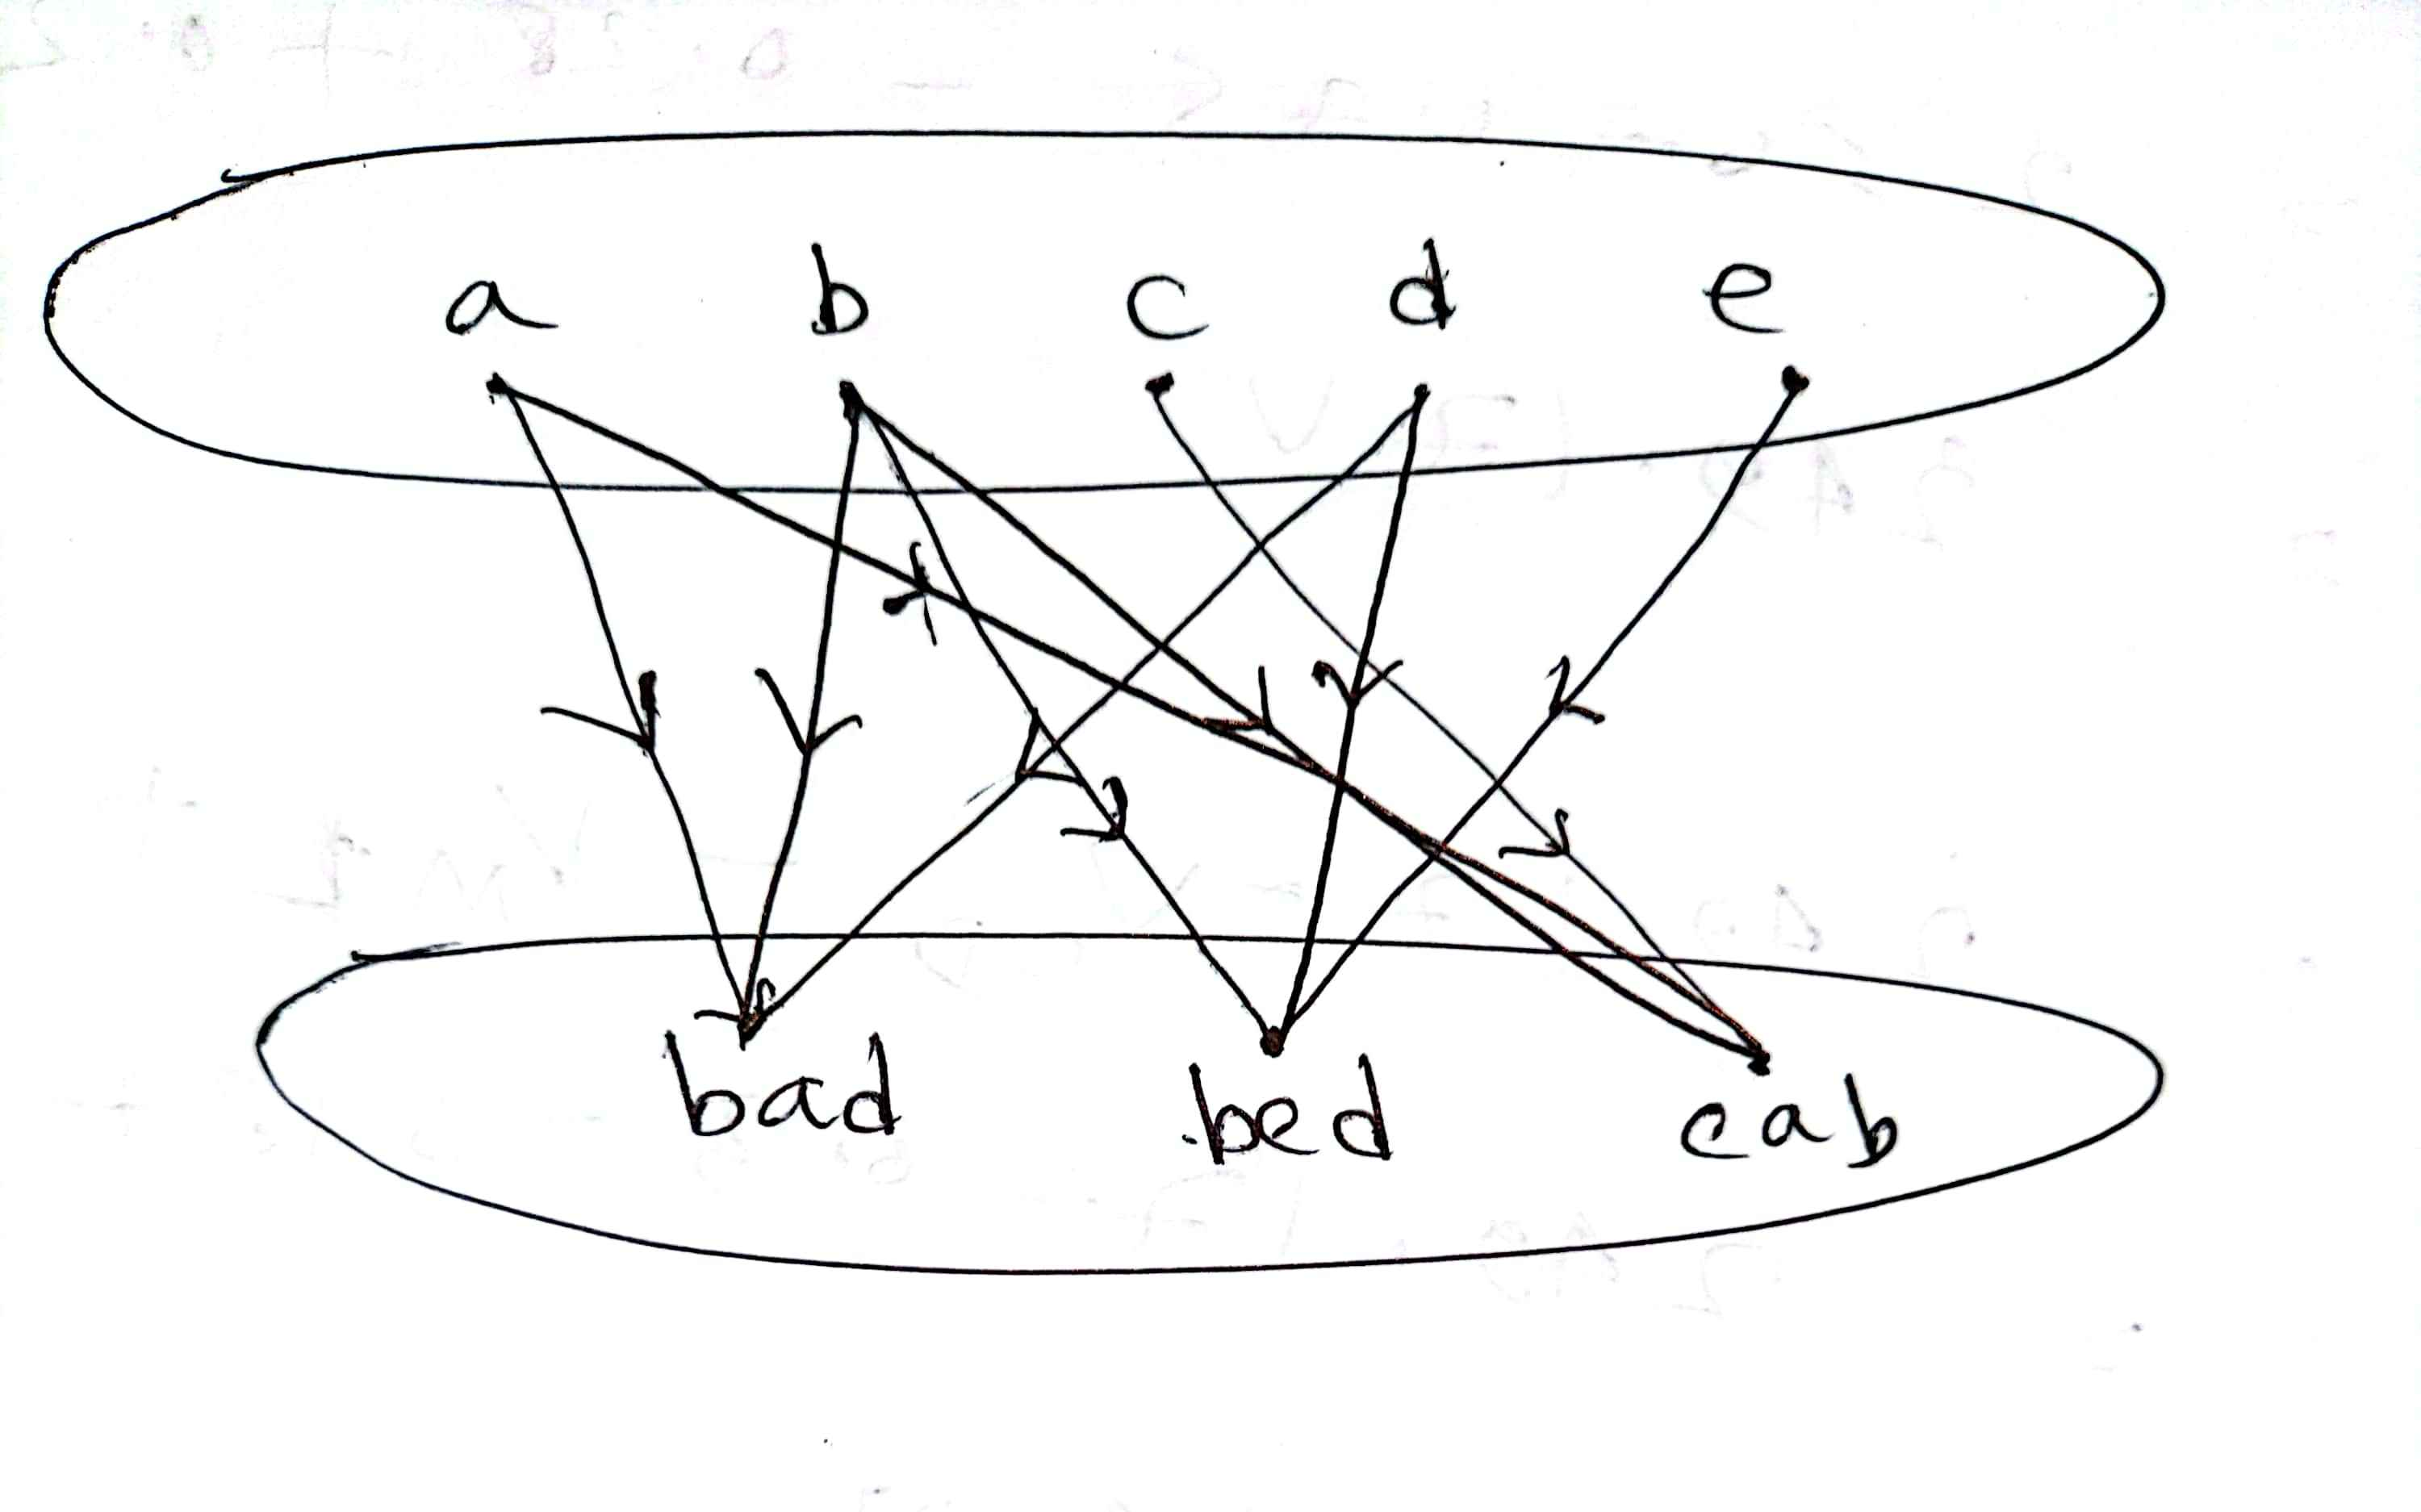
\includegraphics[width=0.5\textwidth]{sol1.jpg}
	\end{figure}
\end{proof}

\begin{exercise}
	{4}
	List the ordered pairs in the relations represented by the directed graphs in Figure 4.4. Determine whether each relation is reflexive, symmetric, or transitive.
	\begin{figure}[H]
		\centering
		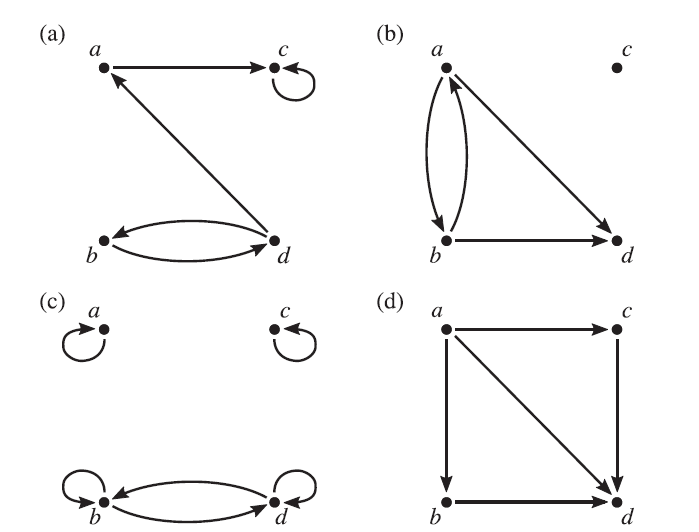
\includegraphics[width=0.5\textwidth]{figure4.4.png}
		\caption*{Figure 4.4}
	\end{figure}
\end{exercise}

\begin{proof}
	(a) $\{(a,c),(c,c),(d,a),(b,d),(d,b)\}$

	i. $a,b, \nd d$ do not have loops. Not reflexive.

	ii. $a,d, \nd a,c$ do not have opposite directional edges towards each other. Not symmetric.

	iii. $d\to a\to c$, but $d\not \to c$. Not transitive.

	(b) $\{(a,b),(b,a),(a,d),(b,d)\}$

	i. None of the vertices has loop. Not reflexive.
	
	ii. $a\to d$ but $d\not \to a$. Not symmetric.

	iii. $a\to b\to a$, but $a\not \to a$. Not transitive.
	
	(c) $\{(a,a), (b,b), (c,c),(d,d),(b,d),(d,b)\}$

	i. Every vertex has loop. It is reflexive.

	ii. Every vertex has either loop or two opposite directional edges or both. It is symmetric.

	iii. $b\to b\to d$ and $b\to d$, and $d\to d\to b$ and $d\to b$. It is transitive.
	
	(d) $\{(a,b),(a,c),(a,d),(b,d),(c,d)\}$

	i. None of the vertices has loop. Not reflexive.

	ii. None of the vertices has two opposite directional edges or loop. Not symmetric.

	iii. $a\to b\to d$ and $b\to d$, $a\to c\to d$ and $a\to d$. It is transitive.       
\end{proof}

\begin{exercise}
	{5}
	Figure 4.5 shows two relations \( R \) and \( S \). Find \( S \circ R \).
	\begin{figure}[H]
		\centering
		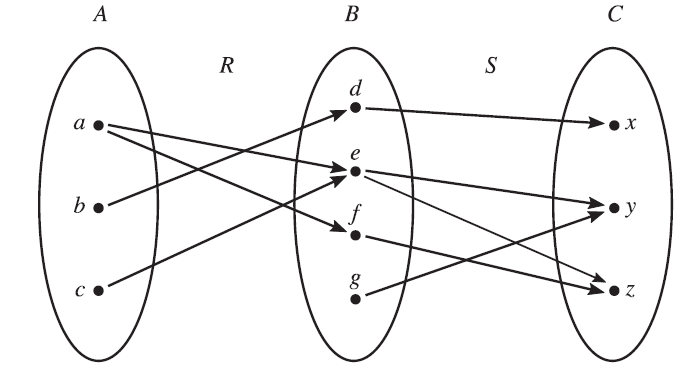
\includegraphics[width=0.5\textwidth]{figure4.5.png}
		\caption*{Figure 4.5}
	\end{figure}
\end{exercise}

\begin{proof}
	$\{(a,y),(a,z),(b,x),(c,y),(c,z)\}$
\end{proof}

\begin{exercise}
	{7}
	Prove part 1 of Theorem 4.3.4.
	\begin{aw}
		\textbf{Theorem 4.3.4.} Suppose \( R \) is a relation on a set \( A \).
		\begin{enumerate}
			\item \( R \) is reflexive if and only if \( i_A \subseteq R \), where as before \( i_A \) is the identity relation on \( A \).
			\item \( R \) is symmetric if and only if \( R = R^{-1} \).
			\item \( R \) is transitive if and only if \( R \circ R \subseteq R \).
		\end{enumerate}
	\end{aw}
\end{exercise}

\begin{proof}
	Suppose $R$ is reflexive on A. Now, by definition, $(x,y)\in i_A$ for all $x,y\in A$ such that $x=y$. Since $R$ is reflexive, $(x,x)\in R$ and so if $x=y$, then $(x,y)\in R$. Thus, $i_A\subseteq R$.
	
	Now we prove the converse. Suppose $i_A\subseteq R$. By definition, $(x,x)\in i_A$ for all $x\in A$ and it follows that $(x,x)\in R$. So, $R$ is reflexive by definition. 
\end{proof}

\begin{exercise}
	{8}
	Prove part 3 of Theorem 4.3.4.
	\begin{aw}
		\textbf{Theorem 4.3.4.} Suppose \( R \) is a relation on a set \( A \).
		\begin{enumerate}
			\item \( R \) is reflexive if and only if \( i_A \subseteq R \), where as before \( i_A \) is the identity relation on \( A \).
			\item \( R \) is symmetric if and only if \( R = R^{-1} \).
			\item \( R \) is transitive if and only if \( R \circ R \subseteq R \).
		\end{enumerate}
	\end{aw}
\end{exercise}

\begin{proof}
	Suppose $R$ is transitive. Now, by definition of composition, if $x,y,z\in A, (x,y)\in R$ and $(y,z)\in R$, then $(x,z)\in R\circ R$. Since $R$ is transitive, $(x,z)\in R$. Thus $R\circ R\subseteq R$.

	Now we prove the converse. Suppose $R\circ R\subseteq R$. So, by definition of composition, if there exists $y\in A$ such that $(x,y)\in R$ and $(y,z)\in R$, then $(x,z)\in R\circ R$. Since $R\circ R\subseteq R$, thus $(x,z)\in R$. Therefore, $R$ is transitive by definition.        
\end{proof}

\begin{exercise}
	{9}
	Suppose \( A \) and \( B \) are sets.
	\begin{enumerate}
		\item[(a)] Show that for every relation \( R \) from \( A \) to \( B \), \( R \circ i_A = R \).
		\item[(b)] Show that for every relation \( R \) from \( A \) to \( B \), \( i_B \circ R = R \).
	\end{enumerate}
\end{exercise}

\begin{proof}
	(a) Let $(a,b)\in R$. By definition, $(a,a)$ must be in $i_A$. So, by definition of composition, we can conclude that $(a,b)\in R\circ i_A$.
	
	Again, let $(a,b)\in R\circ i_A$. By definition of composition, there exists $a\in A$ such that $(a,a)\in i_A$ and $(a,b)\in R$. Thus, $R\circ i_A\subseteq R$, so $R\circ i_A=R$.      
\end{proof}

\begin{exercise}
	{10}
	Suppose \( S \) is a relation on \( A \). Let \( D = \text{Dom}(S) \) and \( R = \text{Ran}(S) \). Prove that \( i_D \subseteq S^{-1} \circ S \) and \( i_R \subseteq S \circ S^{-1} \).
\end{exercise}

\begin{proof}
	$D=\text{Dom}(S)=\{x\in A\mid \exists y\in A \text{ such that } (x,y)\in S\}$ and $i_{D} =\{(x,x)\mid x\in D\}=\{(x,x)\mid \exists y\in A \text{ such that } (x,y)\in S\}$.
	
	Let $(x,x)\in i_{D}$. It implies that there exists $y\in A$ such that $(x,y)\in S$ and so $(y,x)\in S^{-1}$. So, by definition of composition, clearly $(x,x)\in S^{-1}\circ S$. Thus $i_{D} \subseteq S^{-1}\circ S$.
	
	For the second part, $R=\text{Ran}(S)=\{y\in A\mid \exists x\in A \text{ such that } (x,y)\in S\}$ and $i_{R} =\{(y,y)\mid y\in R\}=\{(y,y)\mid \exists x\in A \text{ such that } (x,y)\in S\}$.
	
	Let $(y,y)\in i_{R}$. It implies that there exists $x\in A$ such that $(x,y)\in S$ and so $(y,x)\in S^{-1}$. So, by definition of composition, obviously $(y,y)\in S\circ S^{-1}$. Thus $i_{R} \subseteq S\circ  S^{-1}$.      
\end{proof}

\begin{exercise}
	{11}
	Suppose \( R \) is a relation on \( A \). Prove that if \( R \) is reflexive, then \( R \subseteq R \circ R \).
\end{exercise}

\begin{proof}
	Since $R$ is reflexive on A, by Theorem 4.3.4, $i_A\subseteq R$. By Exercise 14 of Section 4.2, $i_A\circ R\subseteq R\circ R$. By 9(b), we know, $i_A\circ R=R$ and so $R\subseteq R\circ R$.   
\end{proof}

\begin{exercise}
	{12}
	Suppose \( R \) is a relation on \( A \).
	\begin{enumerate}
		\item[(a)] Prove that if \( R \) is reflexive, then so is \( R^{-1} \).
		\item[(b)] Prove that if \( R \) is symmetric, then so is \( R^{-1} \).
		\item[(c)] Prove that if \( R \) is transitive, then so is \( R^{-1} \).
	\end{enumerate}
\end{exercise}

\begin{proof}
	(a) Let $(x,y)\in A\times A$ be an arbitrary ordered pair. Now $(x,y)\in i_A$ for $x=y$ if and only if $(y,x)\in i_{A}^{-1}$ for $x=y$, which can be rewritten as $(x,y)\in i_{A}^{-1}$. So $i_{A} =i_{A}^{-1}$.
	
	Suppose $R$ is reflexive. So $i_{A} \subseteq R$, and it follows that $i_{A} ^{-1}\subseteq R^{-1}$, which is identical to $i_{A} \subseteq R^{-1}$. Hence, $R^{-1}$ is also reflexive.
	
	(b) Suppose $R$ is symmetric. So $R=R^{-1}$. Since $R^{-1} \nd R$ is the same set, thus $R^{-1}$ is also symmetric.
	
	(c) Suppose $R$ is transitive. So $R\circ R\subseteq R$. It implies that $(R\circ R)^{-1} \subseteq R^{-1}$ which further implies that $R^{-1} \circ R^{-1} \subseteq R^{-1}$. So, $R^{-1} $ is also transitive.
\end{proof}

\begin{exercise}
	{13}
	Suppose \( R_1 \) and \( R_2 \) are relations on \( A \). For each part, give either a proof or a counterexample to justify your answer.
	\begin{enumerate}
		\item[(a)] If \( R_1 \) and \( R_2 \) are reflexive, must \( R_1 \cup R_2 \) be reflexive?
		\item[(b)] If \( R_1 \) and \( R_2 \) are symmetric, must \( R_1 \cup R_2 \) be symmetric?
		\item[(c)] If \( R_1 \) and \( R_2 \) are transitive, must \( R_1 \cup R_2 \) be transitive?
	\end{enumerate}
\end{exercise}

\begin{proof}
	(a) Suppose $R_1 \nd R_2$ are reflexive. So $i_{A} \subseteq R_1$ and $i_{A} \subseteq R_2$. Obviously, $i_{A} \subseteq R_1\cup R_2$. So, $R_1\cup R_2$ is also reflexive.
	
	(b) Suppose $R_1 \nd R_2$ are symmetric. So, $R_1=R_1^{-1}$ and $R_2=R_2^{-1} $. Now,
	\[
		R_1\cup R_2=R_1^{-1} \cup R_2^{-1} =(R_1\cup R_2)^{-1}.
	\]
	Thus, $R_1\cup R_2$ is symmetric.
	
	(c) Let $R_1=\{(a,b),(b,d),(a,d)\} \nd R_2=\{(b,a)\}$. So
	\[
		R_1\cup R_2=\{(a,b),(b,d),(a,d),(b,a)\}
	\]
	For $a\to b\to a$, there is no $a\to a$. Therefore, $R_1\cup R_2$ is not transitive.  
\end{proof}

\begin{exercise}
	{14}
	Suppose \( R_1 \) and \( R_2 \) are relations on \( A \). For each part, give either a proof or a counterexample to justify your answer.
	\begin{enumerate}
		\item[(a)] If \( R_1 \) and \( R_2 \) are reflexive, must \( R_1 \cap R_2 \) be reflexive?
		\item[(b)] If \( R_1 \) and \( R_2 \) are symmetric, must \( R_1 \cap R_2 \) be symmetric?
		\item[(c)] If \( R_1 \) and \( R_2 \) are transitive, must \( R_1 \cap R_2 \) be transitive?
	\end{enumerate}
\end{exercise}

\begin{proof}
	(a) Suppose $R_1 \nd R_2$ are reflexive. So, $i_{A} \subseteq R_1$ and $i_{A} \subseteq R_2$. That is, the elements of $i_{A} $ is present in both $R_1 \nd R_2$. Hence, $i_{A} \subseteq R_1\cap R_2$, which implies that $R_1\cap R_2$ is reflexive.
	
	(b) Suppose $R_1$ and $R_2$ are symmetric and so $R_1=R_1^{-1} $ and $R_2=R_2^{-1} $. So
	\[
		R_1\cap R_2=R_1^{-1} \cap R_2^{-1} =(R_1\cap R_2)^{-1} 
	\]
	and it follows that $R_1\cap R_2$ is symmetric.
	
	(c) Suppose $R_1 \nd R_2$ are transitive. By definition of transitivity, if $(a,b) \nd (b,c)$ are in $R_1 \nd R_2$, then $(a,c)$ must be in $R_1 \ro R_2$ respectively. Suppose $(a,b) \nd (b,c)$ are common in $R_1 \nd R_2$. Then $(a,c)$ must be in $R_1$ and $R_2$ both, which implies that $R_1\cap  R_2$ have them all and so it is transitive.           
\end{proof}

\begin{exercise}
	{16}
	Suppose \( R \) and \( S \) are reflexive relations on \( A \). Prove that \( R \circ S \) is reflexive.
\end{exercise}

\begin{proof}
	Suppose $R \nd S$ are reflexive. So, $i_{A} \subseteq R$ and $i_{A} \subseteq S$. Now let $(x,x)\in i_{A} $ for $x\in A$. So $(x,x)\in R$ and $(x,x)\in S$. Then by definition of composition, $(x,x)\in R\circ S$. Hence, $i_{A} \subseteq R\circ S$ and thus $R\circ S$ is reflexive.          
\end{proof}

\begin{exercise}
	{17}
	Suppose \( R \) and \( S \) are symmetric relations on \( A \). Prove that \( R \circ S \) is symmetric if and only if \( R \circ S = S \circ R \).	
\end{exercise}

\begin{proof}
	Suppose $R \nd S$ are symmetric and so $R=R^{-1} $ and $S=S^{-1}$.
	
	Suppose $R\circ S$ is symmetric. So $$R\circ S=(R\circ S)^{-1} =S^{-1} \circ R^{-1} =S\circ R.$$

	Now suppose $R\circ S=S\circ R$. So
	\[
		R\circ S=R^{-1} \circ S^{-1} =(S\circ R)^{-1}.
	\] 
	Therefore, $R\circ S$ is symmetric if and only if $R\circ S=S\circ R$.   
\end{proof}

\begin{exercise}
	{19}
	Consider the following putative theorem.

	\textbf{Theorem?} Suppose \( R \) is a relation on \( A \), and define a relation \( S \) on \( P(A) \) as follows:
	\[
	S = \{ (X, Y) \in P(A) \times P(A) \mid \exists x \in X \, \exists y \in Y \, (x R y) \}.
	\]
	If \( R \) is transitive, then so is \( S \).
	
	(a) What’s wrong with the following proof of the theorem?
	
	\textit{Proof.} Suppose \( R \) is transitive. Suppose \( (X, Y) \in S \) and \( (Y , Z) \in S \). Then by the definition of \( S \), \( x R y \) and \( y R z \), where \( x \in X \), \( y \in Y \), and \( z \in Z \). Since \( x R y \), \( y R z \), and \( R \) is transitive, \( x R z \). But then since \( x \in X \) and \( z \in Z \), it follows from the definition of \( S \) that \( (X, Z) \in S \). Thus, \( S \) is transitive. \qed
	
	(b) Is the theorem correct? Justify your answer with either a proof or a counterexample.
\end{exercise}

\begin{proof}
	(a) ``\( x R y \) and \( y R z \)''-this line is incorrect. Because, $y$ not necessarily need to be the same for $(X,Y)\in S \nd (Y,Z)\in S$.

	(b) Let $R=\{(x,y)\in \mathbb{N}\times \mathbb{N}\mid x\leq y\}$. Here, $R$ is transitive. Now take $X=\{3\}, Y=\{1,3\}, Z=\{2\}\in P(\mathbb{N})$. $(X,Y)\in S \nd (Y,Z)\in S$ since $3R3$ and $1R2$. But $(X,Z)\notin S$ since $3\not\leq 2$.  
\end{proof}

\begin{exercise}
	{22}
	Consider the following putative theorem:

	\textbf{Theorem?} Suppose \( R \) is a relation on \( A \). If \( R \) is symmetric and transitive, then \( R \) is reflexive.

	Is the following proof correct? If so, what proof strategies does it use? If not, can it be fixed? Is the theorem correct?

	\textit{Proof.} Let \( x \) be an arbitrary element of \( A \). Let \( y \) be any element of \( A \) such that \( x R y \). Since \( R \) is symmetric, it follows that \( y R x \). But then by transitivity, since \( x R y \) and \( y R x \), we can conclude that \( x R x \). Since \( x \) was arbitrary, we have shown that \( \forall x \in A \, (x R x) \), so \( R \) is reflexive. \qed
\end{exercise}

\begin{proof}
	No, the proof and theorem neither is correct. Because, it happens so that $x\in A$ but $x\notin \text{Dom}(R)$. And in that case, no such $y$ will be found such that $xRy$ that is done in the proof.
	
	The theorem would be correct if an extra condition that $A=\text{Dom}(R)$ is added to the statement. 
\end{proof}

\begin{exercise}
	{24}
	Let \( R = \{(m, n) \in \mathbb{N} \times \mathbb{N} \mid |m - n| \leq 1 \} \), which is a relation on \( \mathbb{N} \). Note that \( R \subseteq \mathbb{Z} \times \mathbb{Z} \), so \( R \) is also a relation on \( \mathbb{Z} \). This exercise will illustrate why, in part 1 of Definition 4.3.2, we defined the phrase “\( R \) is reflexive on \( A \),” rather than simply “\( R \) is reflexive.”
	\begin{enumerate}
		\item[(a)] Is \( R \) reflexive on \( \mathbb{N} \)?
		\item[(b)] Is \( R \) reflexive on \( \mathbb{Z} \)?
	\end{enumerate}
\end{exercise}

\begin{proof}
	(a) Let $(m,m)$ be an arbitrary ordered pair. Here $\lvert m-m \rvert=0\leq 1$ for all $m\in \mathbb{N}$. Hence, $(m,m)\in R$ and $i_{N} \subseteq R$. So we can conclude that $R$ is reflexive on $\mathbb{N}$.
	
	(b) $R$ is not reflexive on $\mathbb{Z}$. Because, $(-2,-2)\in i_{Z} $, but, as a counterexample, $(-2,-2)\notin R$ since for $(m,n)\in R$, $m,n \in \mathbb{N}$. 
\end{proof}

\section{Section 4.4: Ordering Relations}

\begin{exercise}
	{1}
	In each case, say whether or not \( R \) is a partial order on \( A \). If so, is it a total order?

(a) \( A = \{a, b, c\} \), \( R = \{(a, a), (b, a), (b, b), (b, c), (c, c)\} \).

(b) \( A = \mathbb{R} \), \( R = \{(x, y) \in \mathbb{R} \times \mathbb{R} \mid |x| \leq |y|\} \).

(c) \( A = \mathbb{R} \), \( R = \{(x, y) \in \mathbb{R} \times \mathbb{R} \mid |x| < |y| \text{ or } x = y\} \).
\end{exercise}

\begin{proof}
	
\end{proof}

\begin{exercise}
	{4}
	Suppose \( R \) is a relation on \( A \). You might think that \( R \) could not be both antisymmetric and symmetric, but this isn’t true. Prove that \( R \) is both antisymmetric and symmetric if and only if \( R \subseteq i_A \).
\end{exercise}

\begin{proof}
	
\end{proof}

\begin{exercise}
	{5}
	Suppose \( R \) is a partial order on \( A \) and \( B \subseteq A \). Prove that \( R \cap (B \times B) \) is a partial order on \( B \).
\end{exercise}

\begin{proof}
	
\end{proof}

\begin{exercise}
	{7}
	Suppose \( R_1 \) is a partial order on \( A_1 \), \( R_2 \) is a partial order on \( A_2 \), and \( A_1 \cap A_2 = \emptyset \).

(a) Prove that \( R_1 \cup R_2 \) is a partial order on \( A_1 \cup A_2 \).

(b) Prove that \( R_1 \cup R_2 \cup (A_1 \times A_2) \) is a partial order on \( A_1 \cup A_2 \).

(c) Suppose that \( R_1 \) and \( R_2 \) are total orders. Are the partial orders in parts (a) and (b) also total orders?
\end{exercise}

\begin{proof}
	
\end{proof}

\begin{exercise}
	{8}
	Suppose \( R \) is a partial order on \( A \) and \( S \) is a partial order on \( B \). Define a relation \( T \) on \( A \times B \) as follows:
$T = \{((a, b), (a', b')) \in (A \times B) \times (A \times B) \mid a R a' \text{ and } b S b' \}.$
Show that \( T \) is a partial order on \( A \times B \). If both \( R \) and \( S \) are total orders, will \( T \) also be a total order?
\end{exercise}

\begin{proof}
	
\end{proof}

\begin{exercise}
	{9}
	Suppose \( R \) is a partial order on \( A \) and \( S \) is a partial order on \( B \). Define a relation \( L \) on \( A \times B \) as follows:
$
L = \{((a, b), (a', b')) \in (A \times B) \times (A \times B) \mid a R a', \text{ and if } a = a' \text{ then } b S b' \}.
$
Show that \( L \) is a partial order on \( A \times B \). If both \( R \) and \( S \) are total orders, will \( L \) also be a total order?
\end{exercise}

\begin{proof}
	
\end{proof}
























% --------------------------------------------------------------
%     You don't have to mess with anything below this line.
% --------------------------------------------------------------
\end{document}